\documentclass{article}
\usepackage[utf8]{inputenc}
\usepackage{amsmath, amssymb, amsthm, cancel}
\usepackage{enumitem}
\usepackage{caption}
\usepackage{graphicx}
\usepackage[top=1in, bottom=1in, left=1in, right=1in]{geometry}
\usepackage{float}
\usepackage{booktabs}
\usepackage{array}
\usepackage{multirow}

\title{\textbf{CSCI4150U: Data Mining}\\K-Means and DBSCAN Clustering}
\author{Syed Naqvi \\ Student ID: 100590852}
\date{\today}

\begin{document}

\maketitle

\begin{abstract}
This report analyzes the effectiveness of K-means clustering vs DBSCAN clustering in correctly identifying complex cluster shapes while
using Sum of Squared Errors (SSE) as a measure of cluster compactness. As expected, traditional K-means performed decently in identifying
more globular shaped clusters but struggled with non-globular shapes while DBSCAN was able to identify both globular and non-globular
shapes quite well.
\end{abstract}
    
    

\section{Introduction}

\subsection{Methodology}
We perform the k-means and DBSCAN algorithms on 4 distinct datasets consisting of various shaped clusters, and then compare the effectiveness
of each method. For K-means clustering, model \( k \) values range from 1 to 6 and cluster quality is measured using Sum of Squared Error (SSE)
between points and the cluster centroids. Next, given that our data is 2-dimensional, we start with a \textit{minPts} value of 4 for the
DBSCAN algorithm and then use k-distance plots to estimate ideal \textbf{eps} values. The \textit{minPts} and \textbf{eps} values are further
adjusted using trial and error.

\subsection{Preprocessing}
To initialize our dataset for clustering, we perform feature standardization and remove the existing labels
column giving the following initial plots:
\begin{figure}[H]
    \centering
    \begin{minipage}[b]{0.49\textwidth}
        \centering
        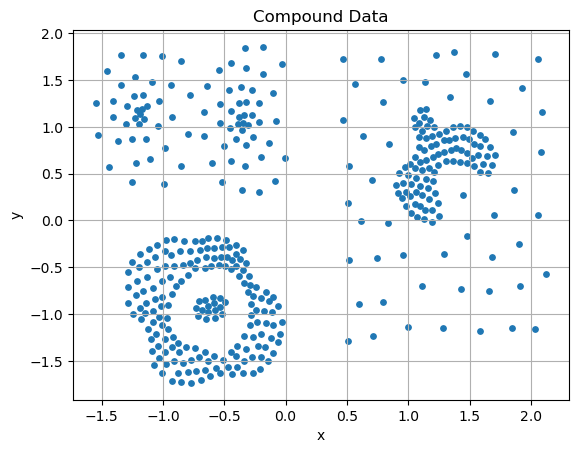
\includegraphics[width=\textwidth]{ea.png}
        \caption{Compound Data}
    \end{minipage}
    \hfill
    \begin{minipage}[b]{0.49\textwidth}
        \centering
        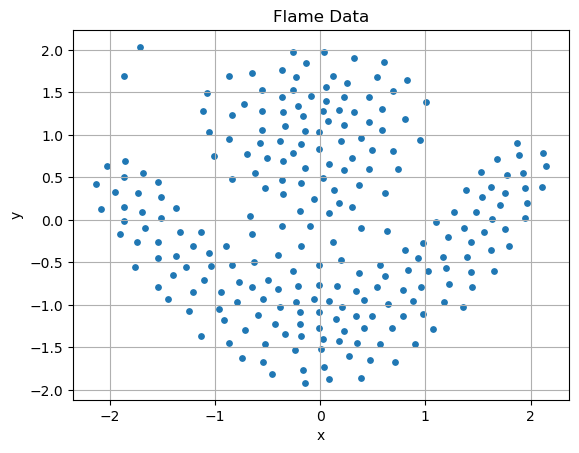
\includegraphics[width=\textwidth]{eb.png}
        \caption{Flame Data}
    \end{minipage}
\end{figure}
\begin{figure}[H]
    \centering
    \begin{minipage}[b]{0.49\textwidth}
        \centering
        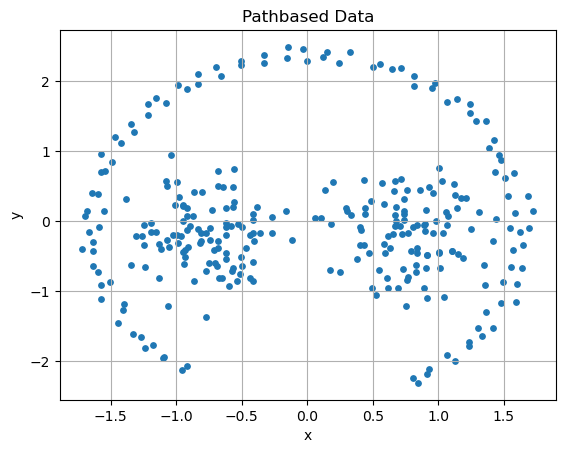
\includegraphics[width=\textwidth]{ec.png}
        \caption{Pathbased Data}
    \end{minipage}
    \hfill
    \begin{minipage}[b]{0.49\textwidth}
        \centering
        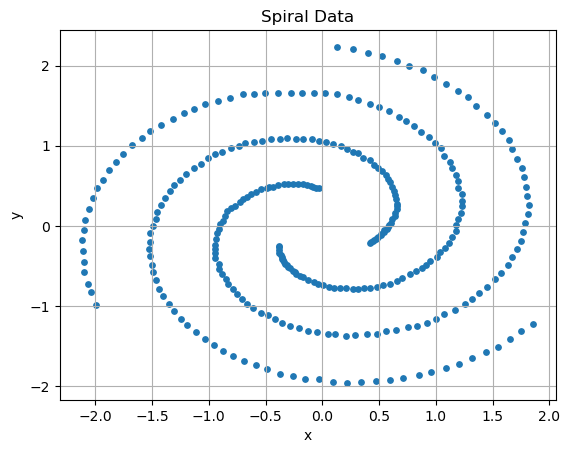
\includegraphics[width=\textwidth]{ed.png}
        \caption{Spiral Data}
    \end{minipage}
\end{figure}

\section{Part I:}
\subsection{K-Means Clustering}
\begin{figure}[H]
    \centering
    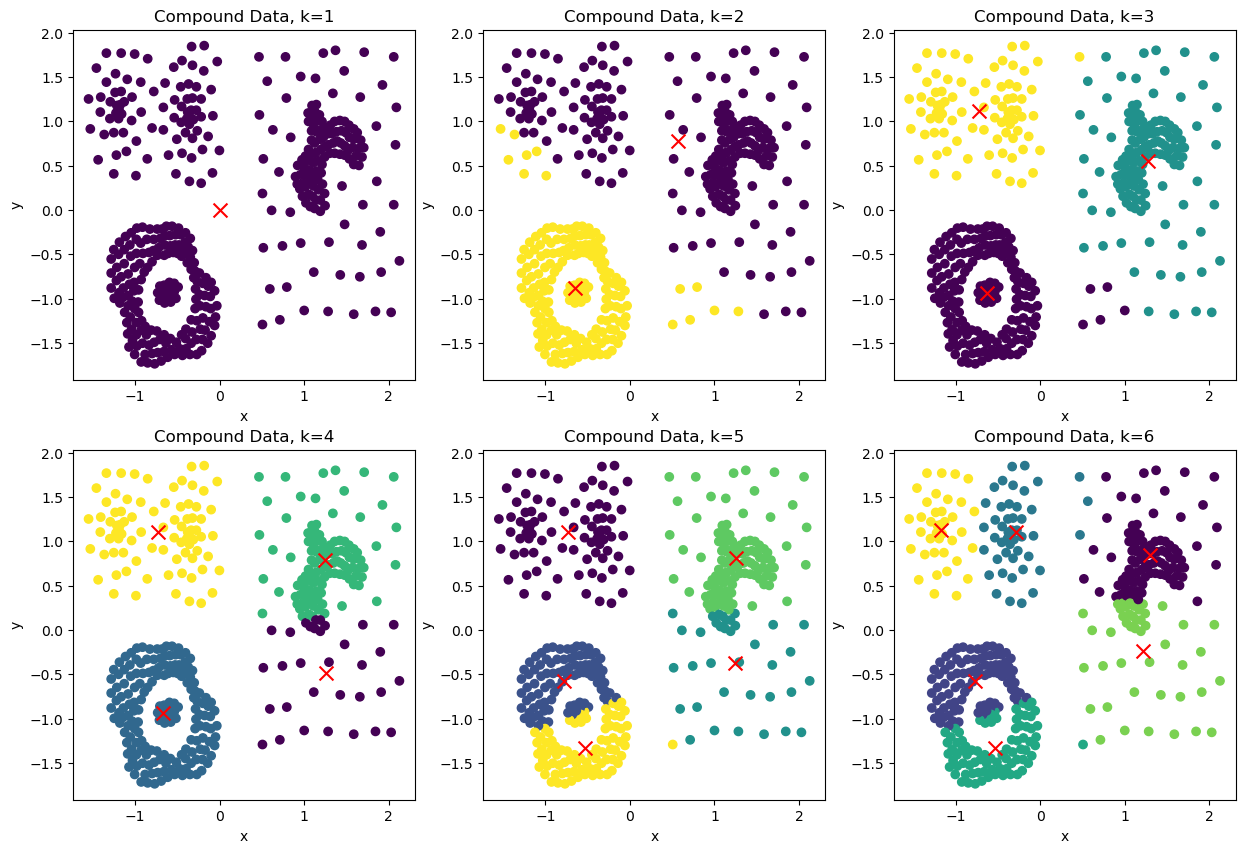
\includegraphics[width=\textwidth]{compound_p.png}
    \caption{Compound Data Clustering}
\end{figure}
\begin{figure}[H]
    \centering
    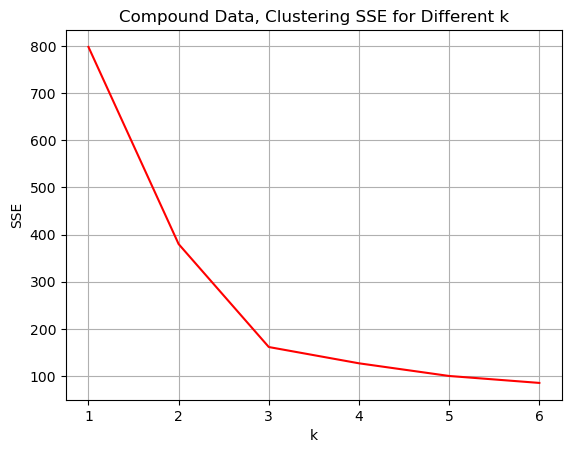
\includegraphics[width=0.6\textwidth]{compound_s.png}
    \caption{Compound Data SSE for Different k}
\end{figure}
\begin{figure}[H]
    \centering
    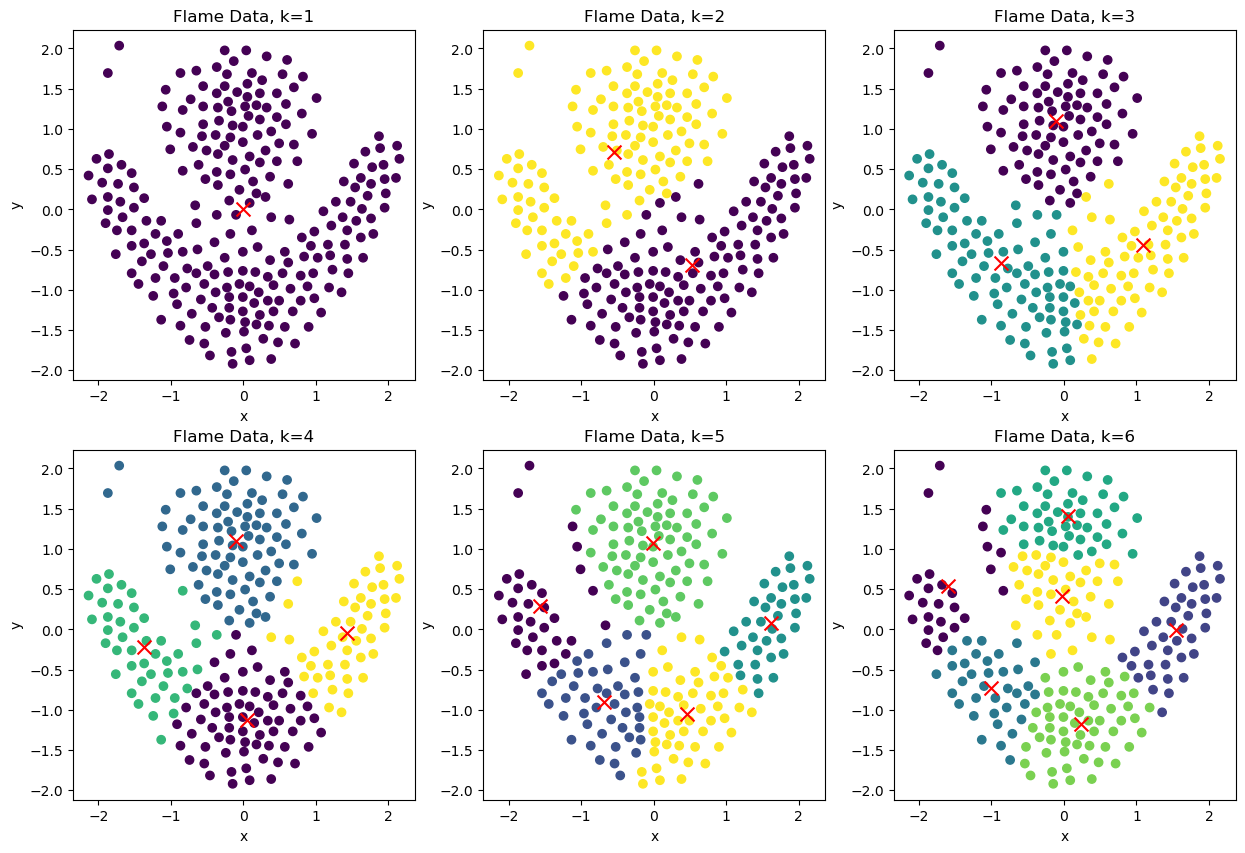
\includegraphics[width=\textwidth]{flame_p.png}
    \caption{Flame Data Clustering}
\end{figure}
\begin{figure}[H]
    \centering
    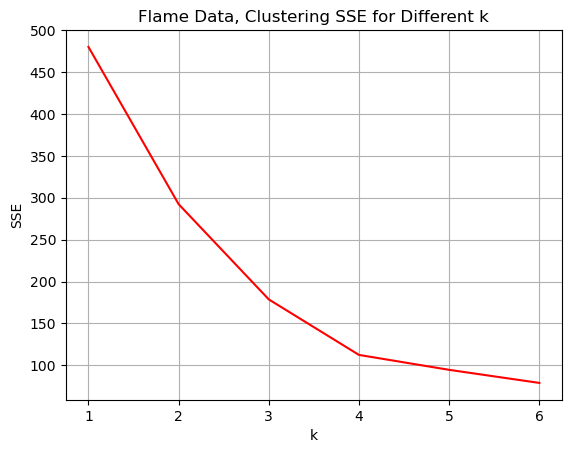
\includegraphics[width=0.6\textwidth]{flame_s.png}
    \caption{Flame Data SSE for Different k}
\end{figure}
\begin{figure}[H]
    \centering
    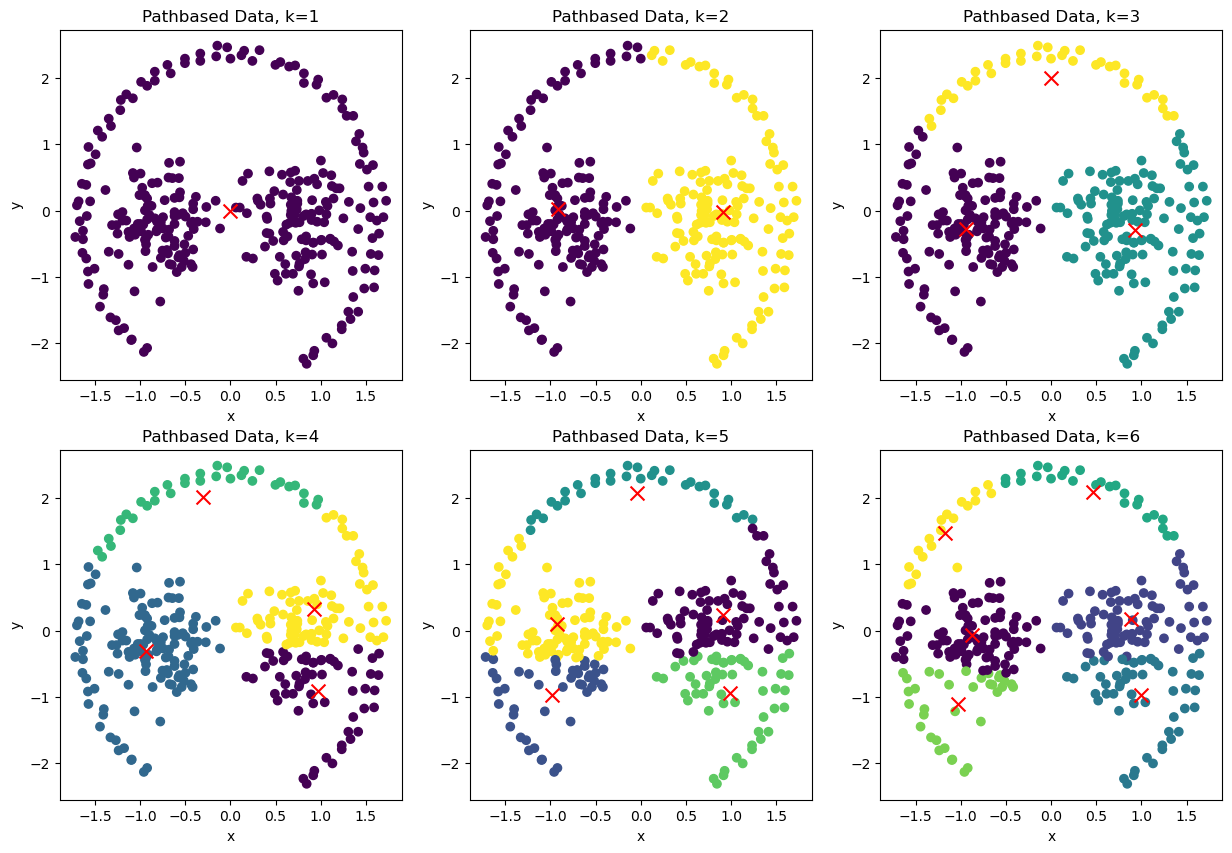
\includegraphics[width=\textwidth]{pathbased_p.png}
    \caption{Pathbased Data Clustering}
\end{figure}
\begin{figure}[H]
    \centering
    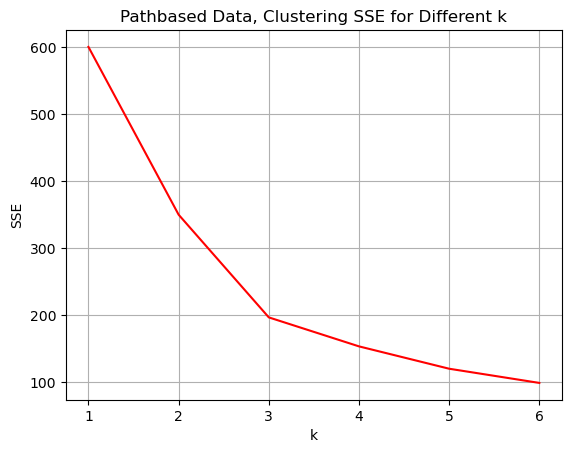
\includegraphics[width=0.6\textwidth]{pathbased_s.png}
    \caption{Pathbased Data SSE for Different k}
\end{figure}
\begin{figure}[H]
    \centering
    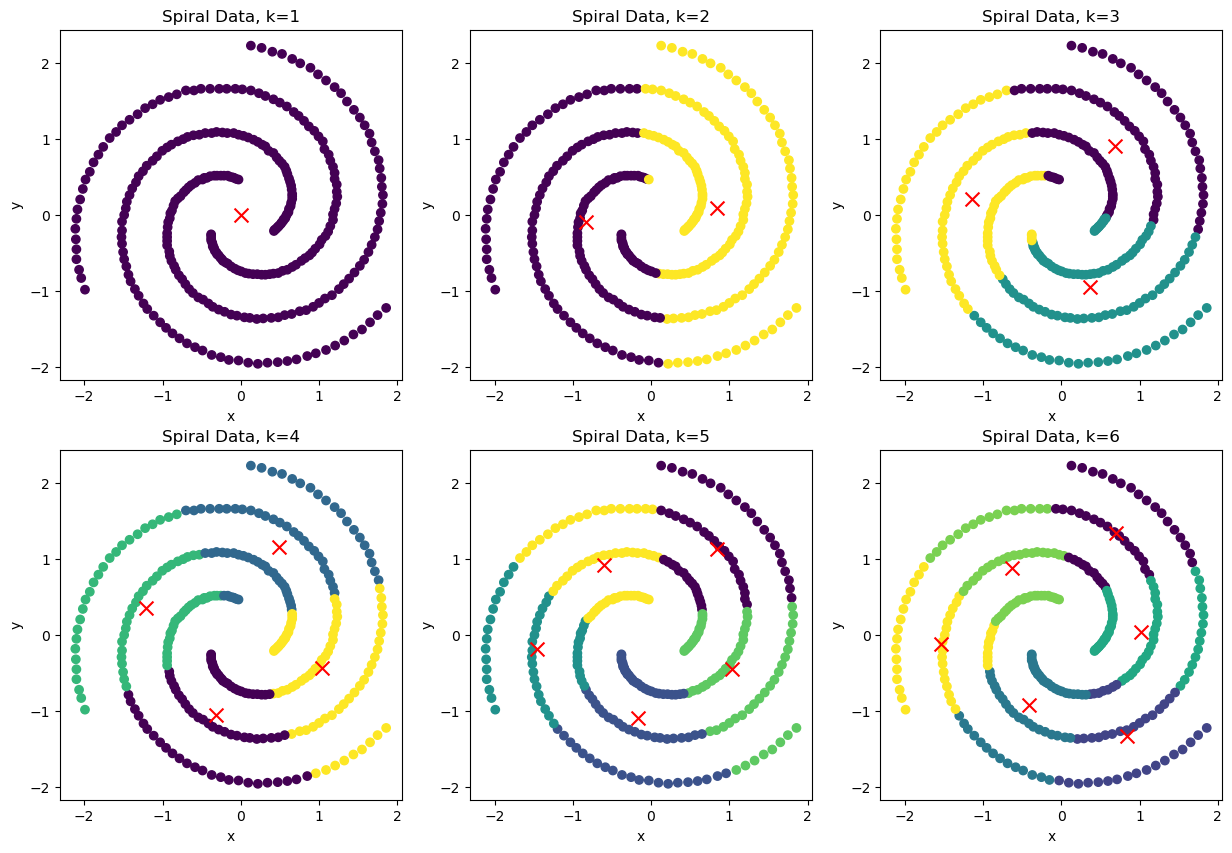
\includegraphics[width=\textwidth]{spiral_p.png}
    \caption{Compound Data Clustering}
\end{figure}
\begin{figure}[H]
    \centering
    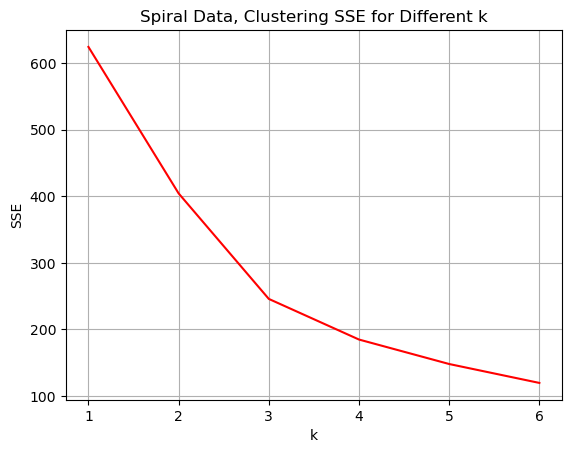
\includegraphics[width=0.6\textwidth]{spiral_s.png}
    \caption{Spiral Data SSE for Different k}
\end{figure}

\subsection{Conclusion}
From the above figures it becomes clear that simply reducing the raw SSE score is not always the best
way to determine the ideal number of clusters. This is because increasing the number of clusters, even
if they are not accurately representing true groupings in the data will still reduce the SSE. This is
most evident in the above plots where despite the SSE measures following the familiar 'elbow' curves,
none of the corresponding clusters can accurately distinguish spiral arms in the Spiral dataset,
the outer 'containing' cluster at the bottom left of the Compound Dataset or the border of the Pathbased
dataset. Even though k-means cannot distinguish between complex cluster shapes, using centroids to
approximate globular shaped clusters seems to work best when k=3 for all the datasets.   

\newpage

\section{Part II: DBSCAN}

First, we use a random value assignment for \textit{minPts} and \textit{eps} to get a sense of the
performance of the DBSCAN algorithm: 
\begin{figure}[H]
    \centering
    \begin{minipage}[b]{0.49\textwidth}
        \centering
        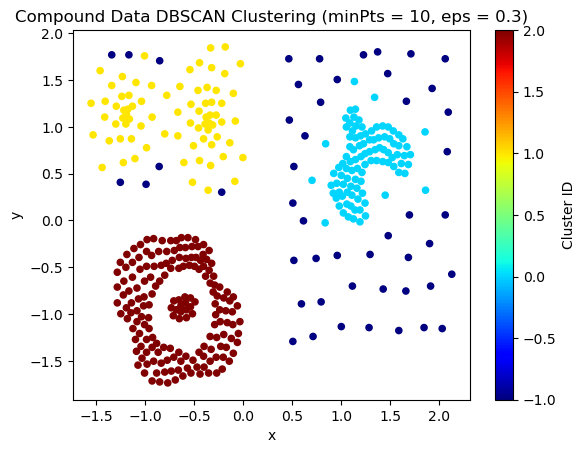
\includegraphics[width=\textwidth]{DB_rand_compund.png}
        \caption{DBSCAN Compound Data}
    \end{minipage}
    \hfill
    \begin{minipage}[b]{0.49\textwidth}
        \centering
        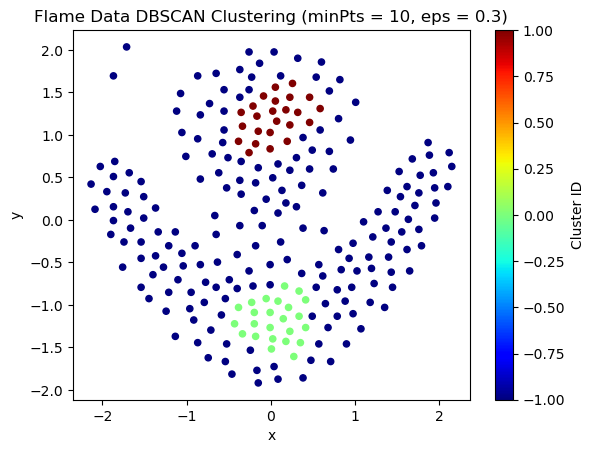
\includegraphics[width=\textwidth]{DB_rand_flame.png}
        \caption{DBSCAN Flame Data}
    \end{minipage}
\end{figure}
\begin{figure}[H]
    \centering
    \begin{minipage}[b]{0.49\textwidth}
        \centering
        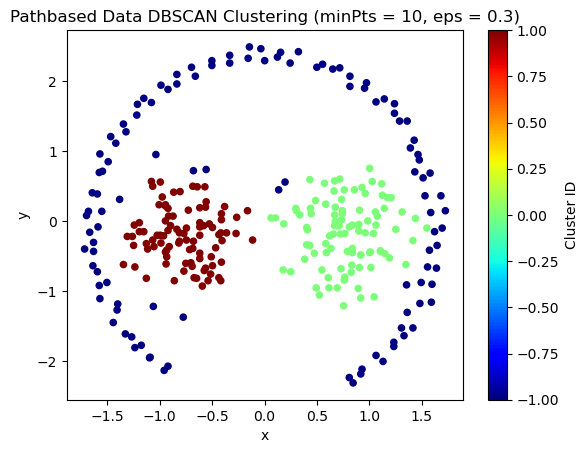
\includegraphics[width=\textwidth]{DB_rand_pathbased.png}
        \caption{DBSCAN Pathbased Data}
    \end{minipage}
    \hfill
    \begin{minipage}[b]{0.49\textwidth}
        \centering
        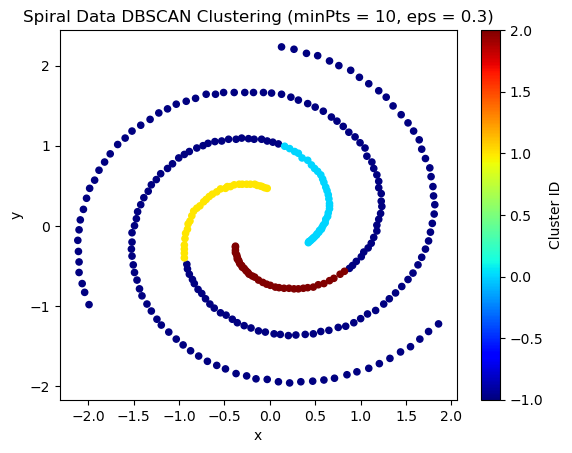
\includegraphics[width=\textwidth]{DB_rand_spiral.png}
        \caption{DBSCAN Spiral Data}
    \end{minipage}
\end{figure}

Next, we can use k-distance plots and some trial and error to arrive at the ideal parameters values that
result in the best clustering for all datasets:

\begin{figure}[H]
    \centering
    \begin{minipage}[b]{0.49\textwidth}
        \centering
        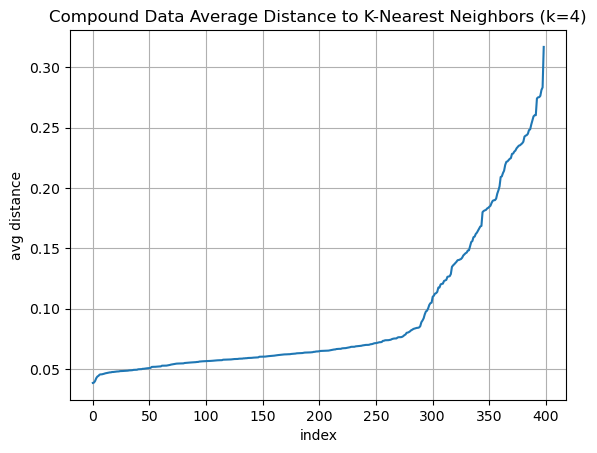
\includegraphics[width=\textwidth]{k_dist_compound.png}
        \caption{K-Distance Plot Compound Data}
    \end{minipage}
    \hfill
    \begin{minipage}[b]{0.49\textwidth}
        \centering
        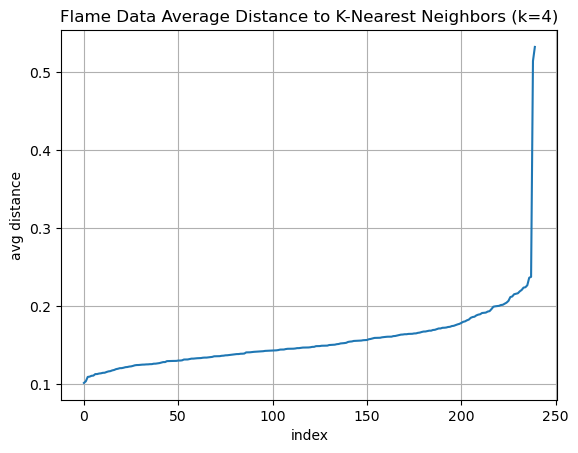
\includegraphics[width=\textwidth]{k_dist_flame.png}
        \caption{K-Distance Plot Flame Data}
    \end{minipage}
\end{figure}
\begin{figure}[H]
    \centering
    \begin{minipage}[b]{0.49\textwidth}
        \centering
        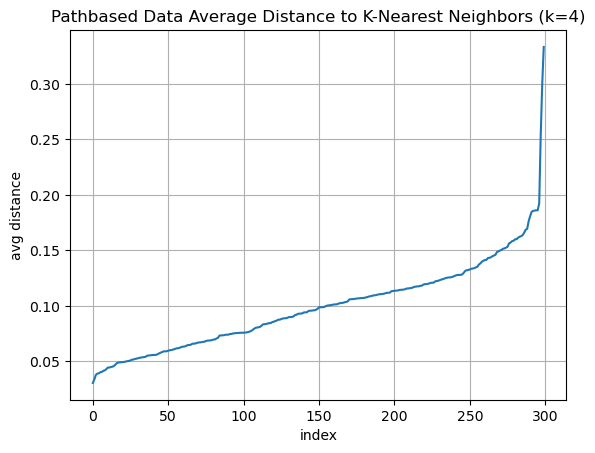
\includegraphics[width=\textwidth]{k_dist_pathbased.png}
        \caption{K-Distance Plot Pathbased Data}
    \end{minipage}
    \hfill
    \begin{minipage}[b]{0.49\textwidth}
        \centering
        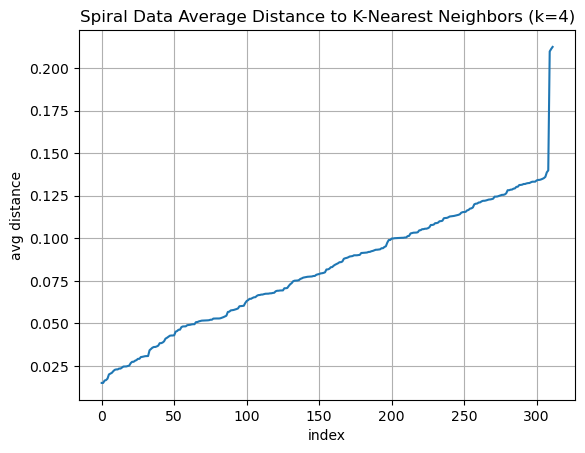
\includegraphics[width=\textwidth]{k_dist_spiral.png}
        \caption{K-Distance Plot Spiral Data}
    \end{minipage}
\end{figure}

\begin{figure}[H]
    \centering
    \begin{minipage}[b]{0.49\textwidth}
        \centering
        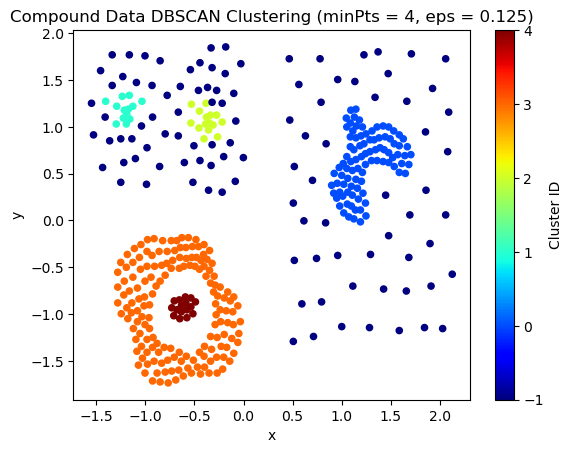
\includegraphics[width=\textwidth]{DB_final_compund.png}
        \caption{DBSCAN Final Clusters Compound Data}
    \end{minipage}
    \hfill
    \begin{minipage}[b]{0.49\textwidth}
        \centering
        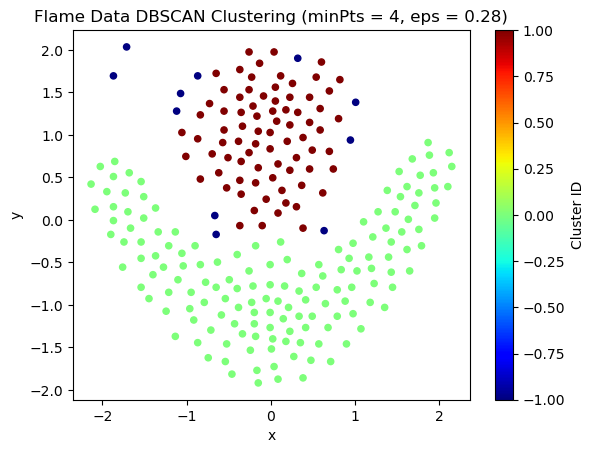
\includegraphics[width=\textwidth]{DB_final_flame.png}
        \caption{DBSCAN Final Clusters Flame Data}
    \end{minipage}
\end{figure}
\begin{figure}[H]
    \centering
    \begin{minipage}[b]{0.49\textwidth}
        \centering
        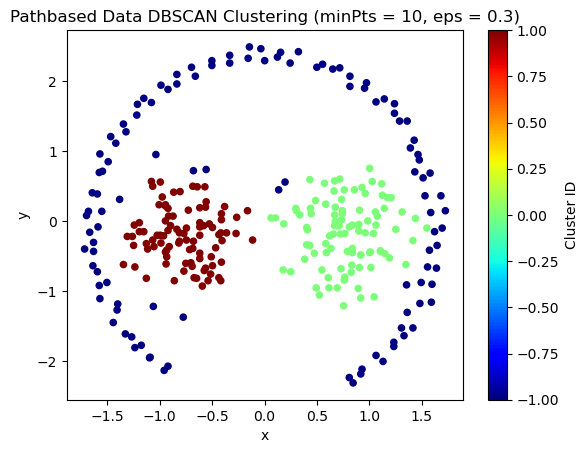
\includegraphics[width=\textwidth]{DB_final_pathbased.png}
        \caption{DBSCAN Final Clusters Pathbased Data}
    \end{minipage}
    \hfill
    \begin{minipage}[b]{0.49\textwidth}
        \centering
        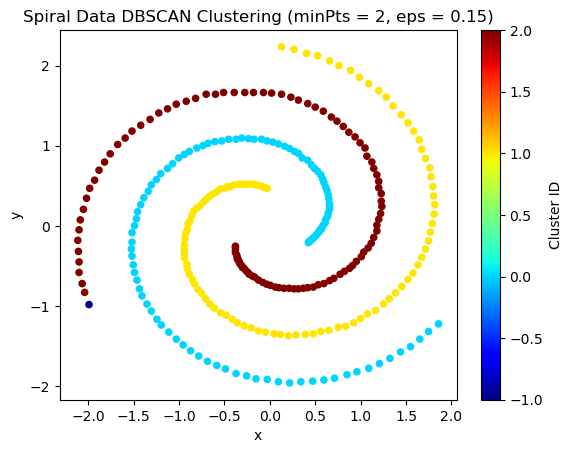
\includegraphics[width=\textwidth]{DB_final_spiral.png}
        \caption{DBSCAN Final Clusters Spiral Data}
    \end{minipage}
\end{figure}

\subsection{Conclusion}
We can see that DBSCAN, with some effort in parameter selection, performs very well in identifying
clusters at a level most humans would find intuitive. The denisty based approach is much more flexible
in finding complex cluster shapes as opposed to centroid based clustering which only works well in
globular regional partitioning. Even if a particular region may contain multiple non-globular shaped
clusters, k-means would try to partition the region to fit the globular mold.

\end{document}
